% Options for packages loaded elsewhere
\PassOptionsToPackage{unicode}{hyperref}
\PassOptionsToPackage{hyphens}{url}
%
\documentclass[
  ignorenonframetext,
]{beamer}
\usepackage{pgfpages}
\setbeamertemplate{caption}[numbered]
\setbeamertemplate{caption label separator}{: }
\setbeamercolor{caption name}{fg=normal text.fg}
\beamertemplatenavigationsymbolsempty
% Prevent slide breaks in the middle of a paragraph
\widowpenalties 1 10000
\raggedbottom
\setbeamertemplate{part page}{
  \centering
  \begin{beamercolorbox}[sep=16pt,center]{part title}
    \usebeamerfont{part title}\insertpart\par
  \end{beamercolorbox}
}
\setbeamertemplate{section page}{
  \centering
  \begin{beamercolorbox}[sep=12pt,center]{part title}
    \usebeamerfont{section title}\insertsection\par
  \end{beamercolorbox}
}
\setbeamertemplate{subsection page}{
  \centering
  \begin{beamercolorbox}[sep=8pt,center]{part title}
    \usebeamerfont{subsection title}\insertsubsection\par
  \end{beamercolorbox}
}
\AtBeginPart{
  \frame{\partpage}
}
\AtBeginSection{
  \ifbibliography
  \else
    \frame{\sectionpage}
  \fi
}
\AtBeginSubsection{
  \frame{\subsectionpage}
}
\usepackage{amsmath,amssymb}
\usepackage{lmodern}
\usepackage{iftex}
\ifPDFTeX
  \usepackage[T1]{fontenc}
  \usepackage[utf8]{inputenc}
  \usepackage{textcomp} % provide euro and other symbols
\else % if luatex or xetex
  \usepackage{unicode-math}
  \defaultfontfeatures{Scale=MatchLowercase}
  \defaultfontfeatures[\rmfamily]{Ligatures=TeX,Scale=1}
\fi
% Use upquote if available, for straight quotes in verbatim environments
\IfFileExists{upquote.sty}{\usepackage{upquote}}{}
\IfFileExists{microtype.sty}{% use microtype if available
  \usepackage[]{microtype}
  \UseMicrotypeSet[protrusion]{basicmath} % disable protrusion for tt fonts
}{}
\makeatletter
\@ifundefined{KOMAClassName}{% if non-KOMA class
  \IfFileExists{parskip.sty}{%
    \usepackage{parskip}
  }{% else
    \setlength{\parindent}{0pt}
    \setlength{\parskip}{6pt plus 2pt minus 1pt}}
}{% if KOMA class
  \KOMAoptions{parskip=half}}
\makeatother
\usepackage{xcolor}
\newif\ifbibliography
\usepackage{graphicx}
\makeatletter
\def\maxwidth{\ifdim\Gin@nat@width>\linewidth\linewidth\else\Gin@nat@width\fi}
\def\maxheight{\ifdim\Gin@nat@height>\textheight\textheight\else\Gin@nat@height\fi}
\makeatother
% Scale images if necessary, so that they will not overflow the page
% margins by default, and it is still possible to overwrite the defaults
% using explicit options in \includegraphics[width, height, ...]{}
\setkeys{Gin}{width=\maxwidth,height=\maxheight,keepaspectratio}
% Set default figure placement to htbp
\makeatletter
\def\fps@figure{htbp}
\makeatother
\setlength{\emergencystretch}{3em} % prevent overfull lines
\providecommand{\tightlist}{%
  \setlength{\itemsep}{0pt}\setlength{\parskip}{0pt}}
\setcounter{secnumdepth}{-\maxdimen} % remove section numbering
\ifLuaTeX
  \usepackage{selnolig}  % disable illegal ligatures
\fi
\IfFileExists{bookmark.sty}{\usepackage{bookmark}}{\usepackage{hyperref}}
\IfFileExists{xurl.sty}{\usepackage{xurl}}{} % add URL line breaks if available
\urlstyle{same} % disable monospaced font for URLs
\hypersetup{
  pdftitle={DTE Interim},
  hidelinks,
  pdfcreator={LaTeX via pandoc}}

\title{DTE Interim}
\author{}
\date{\vspace{-2.5em}2022-11-23}

\begin{document}
\frame{\titlepage}

\begin{frame}{Set-up}
\protect\hypertarget{set-up}{}
We are planning a survival trial in which we are anticipating there to
be delayed treatment effects (DTE). We have elicited two prior
distributions:

\begin{itemize}
\tightlist
\item
  For \(T\), the length of delay
\item
  For HR, the post-delay hazard ratio
\end{itemize}

How can we use these elicited prior distributions to help us decide
when/if to perform any interim analysis?

Given some data, and these elicited prior distributions, we are able to
calculate the posterior distributions for both \(T\) and HR.
\end{frame}

\begin{frame}{Calculating posteriors}
\protect\hypertarget{calculating-posteriors}{}
\(T \sim N(6, 2.97^2)\) HR \(\sim\) Be(10.8, 6.87)

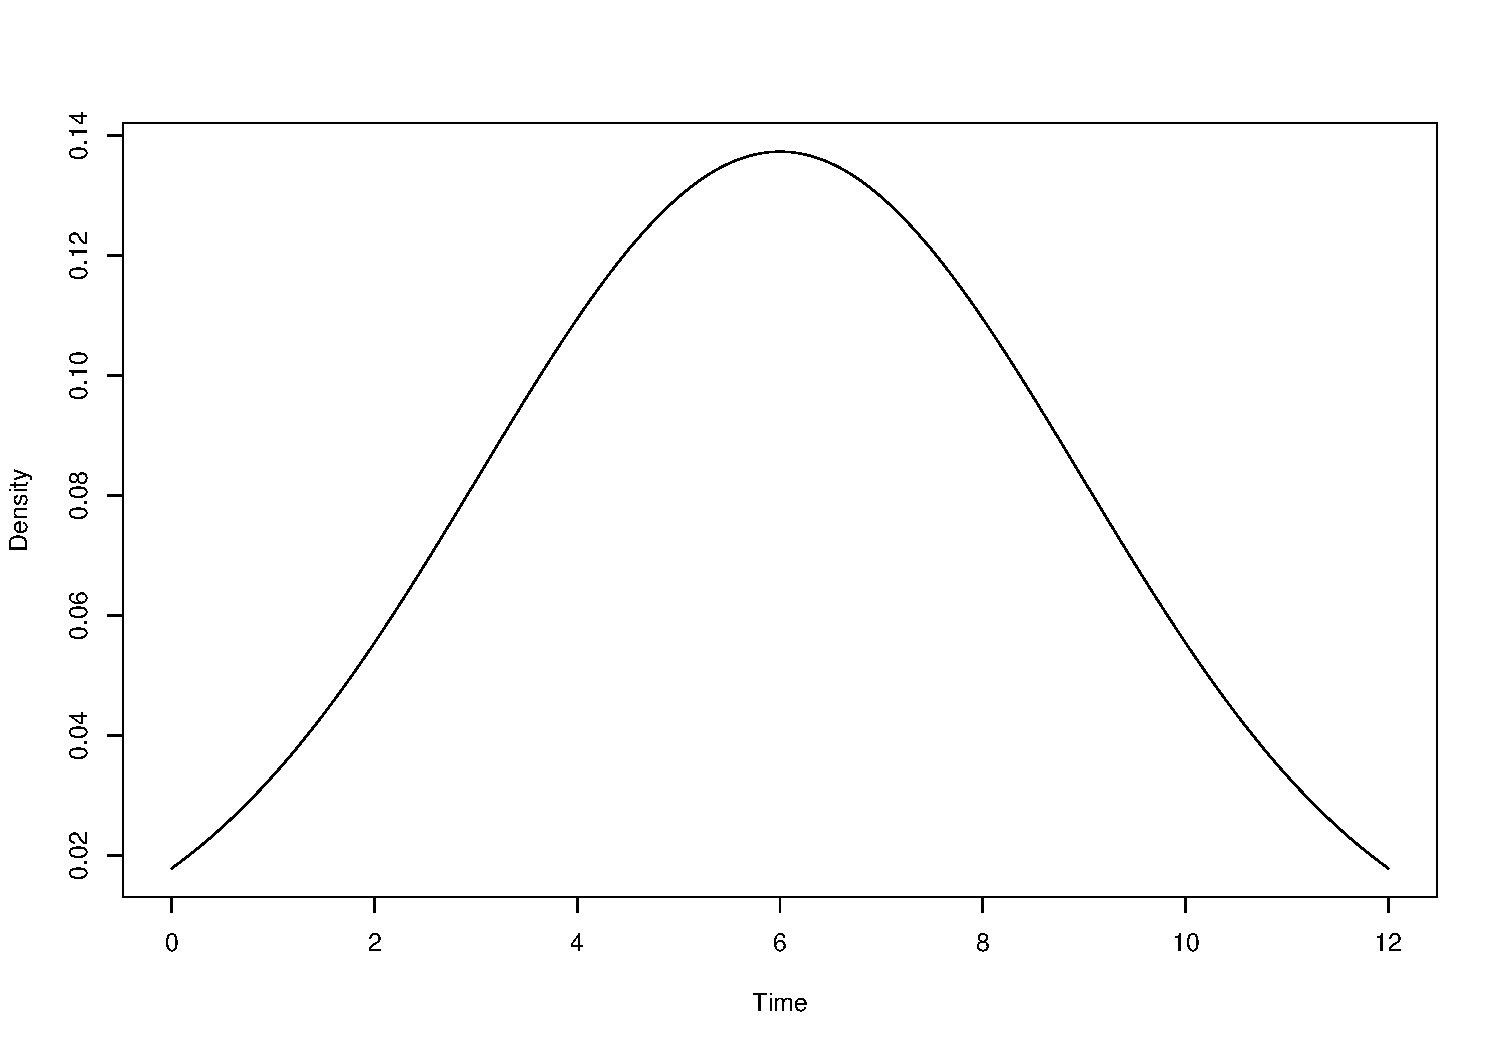
\includegraphics{DTEInterim_files/figure-beamer/priors-1.pdf}

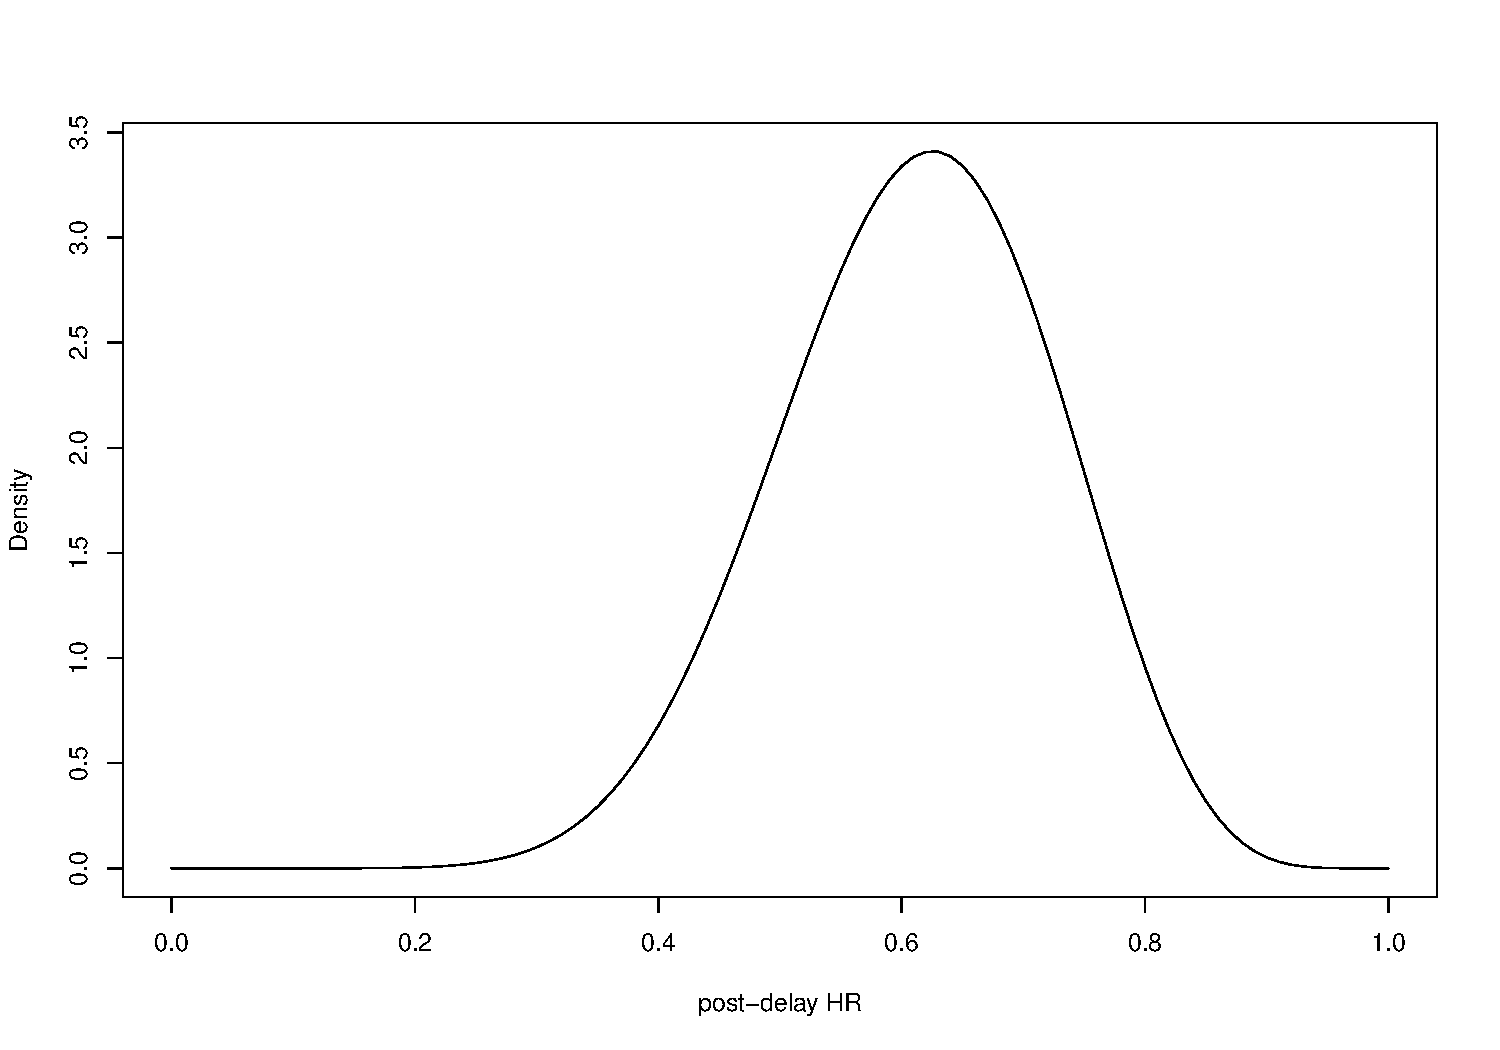
\includegraphics{DTEInterim_files/figure-beamer/prior HR-1.pdf}

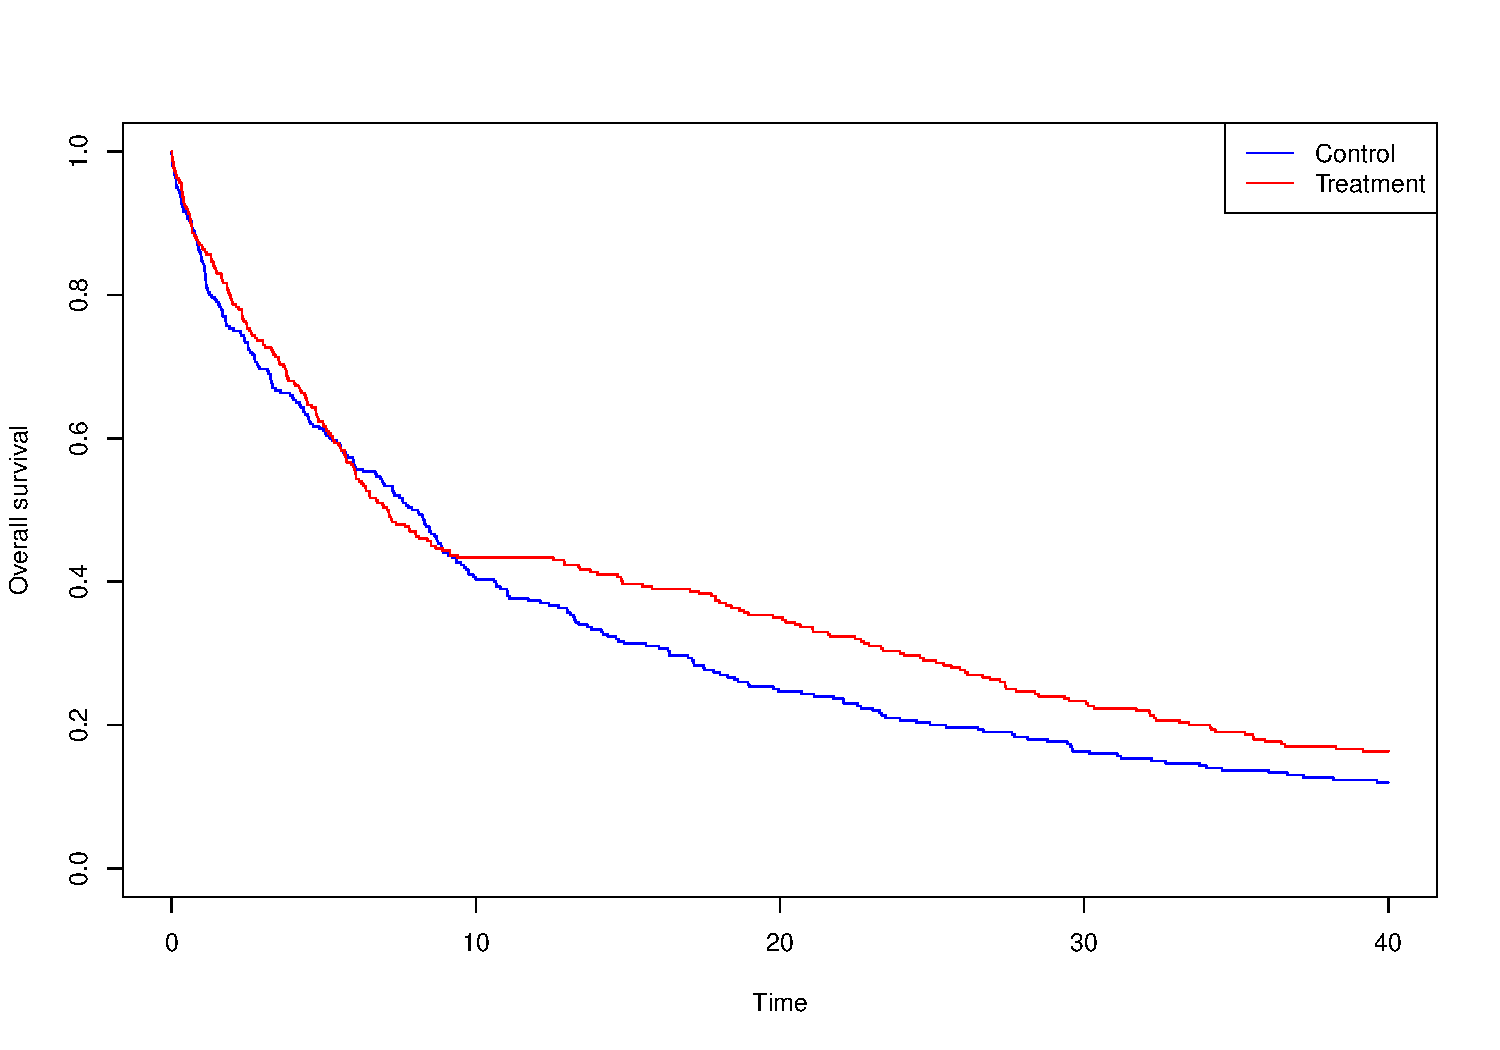
\includegraphics{DTEInterim_files/figure-beamer/data-1.pdf}

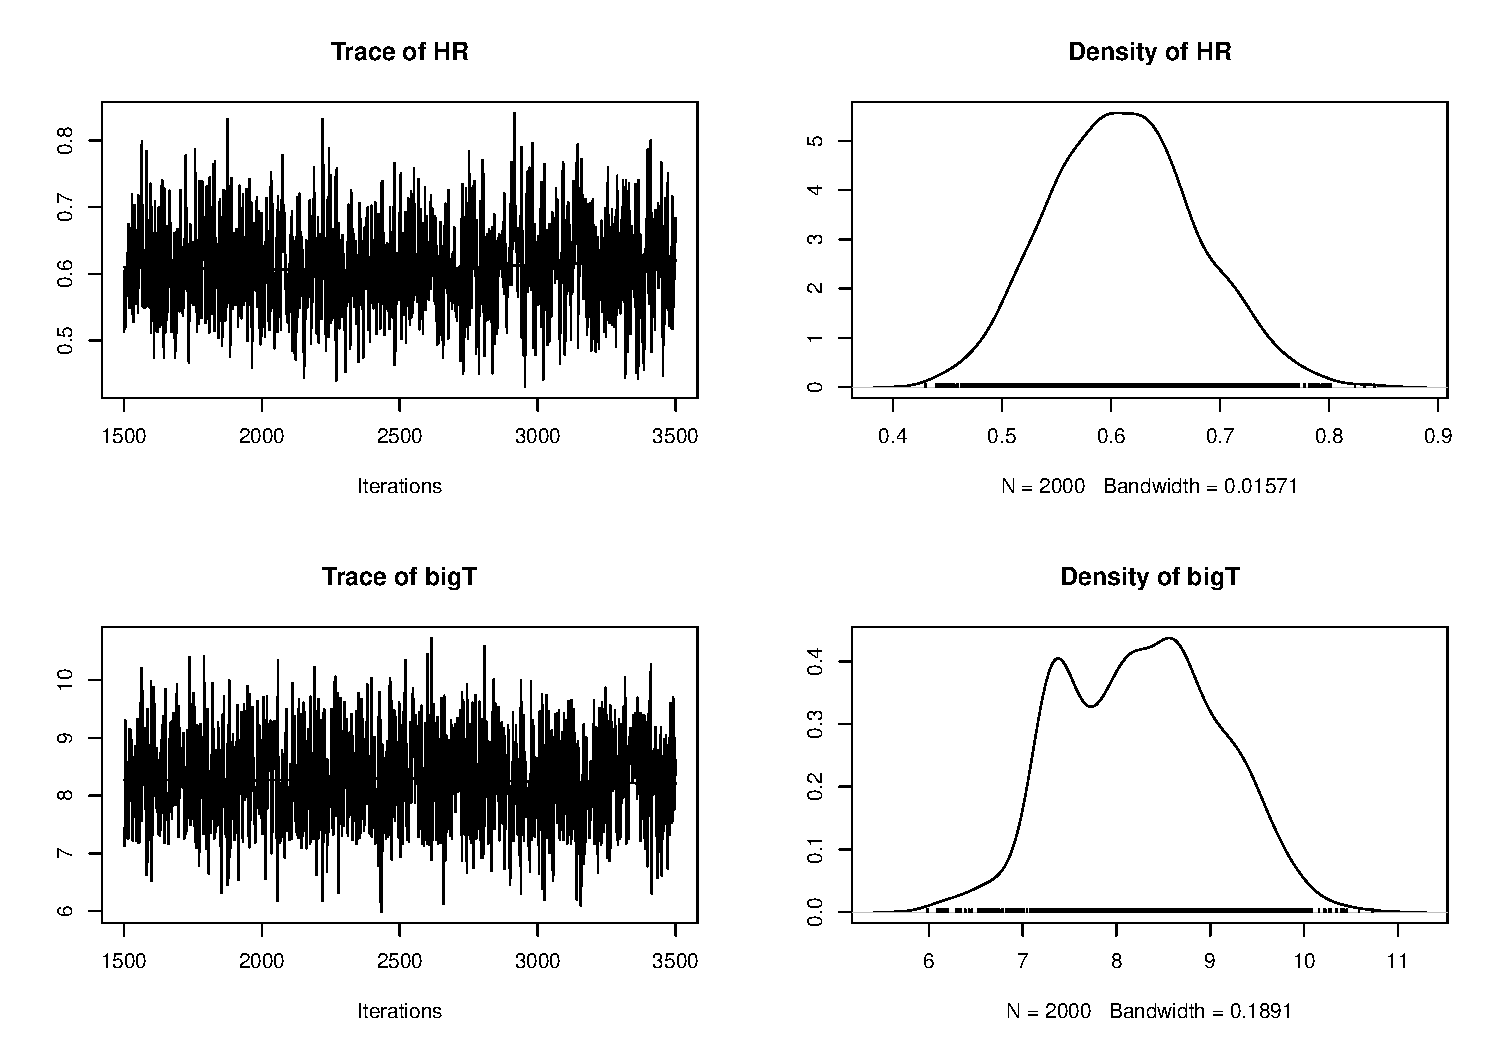
\includegraphics{DTEInterim_files/figure-beamer/posteriors-1.pdf}
\end{frame}

\begin{frame}{Set-up}
\protect\hypertarget{set-up-1}{}
Now we have this mechanism, how can we use it to investigate the problem
of choosing the `optimum' time to perform an interim analysis? What do
these posteriors tell us?

We can change the interim analysis time and see what effect this has on
the posteriors. We hypothesize that as we increase the IA time, the
posterior for the HR will be more concentrated around the ``true''
value.

To investigate this, we choose some target effect and calculate the
proportion of the posterior which is less than this target value.
\end{frame}

\begin{frame}{Set-up}
\protect\hypertarget{set-up-2}{}
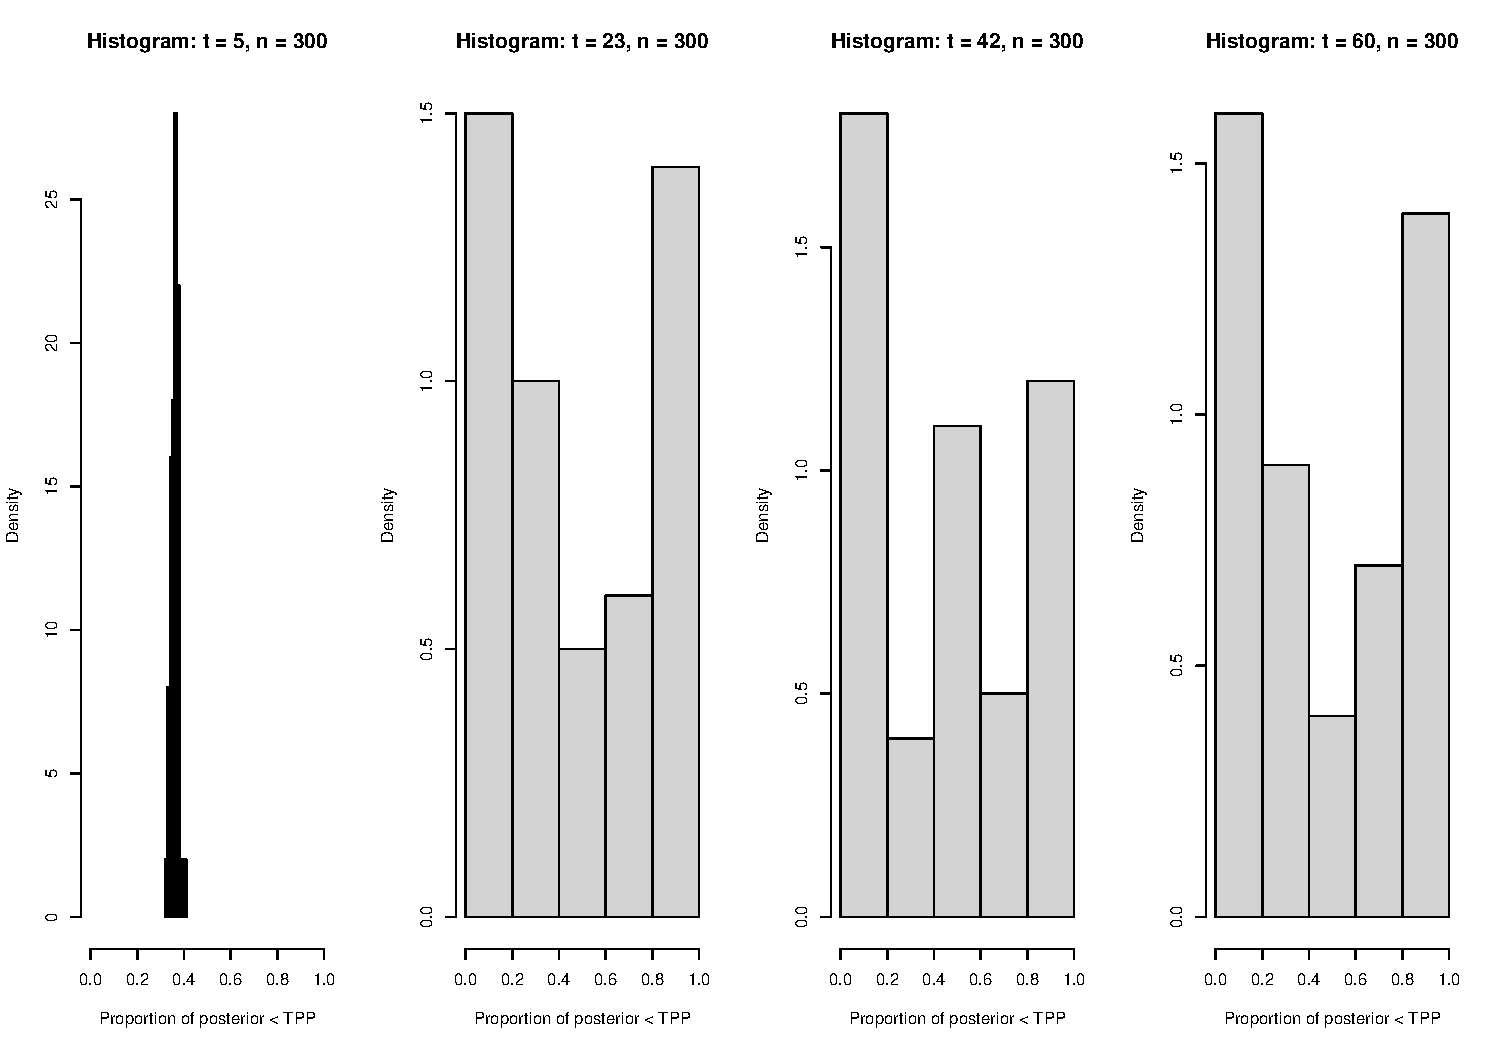
\includegraphics{DTEInterim_files/figure-beamer/unnamed-chunk-1-1.pdf}
\end{frame}

\begin{frame}{Set-up}
\protect\hypertarget{set-up-3}{}
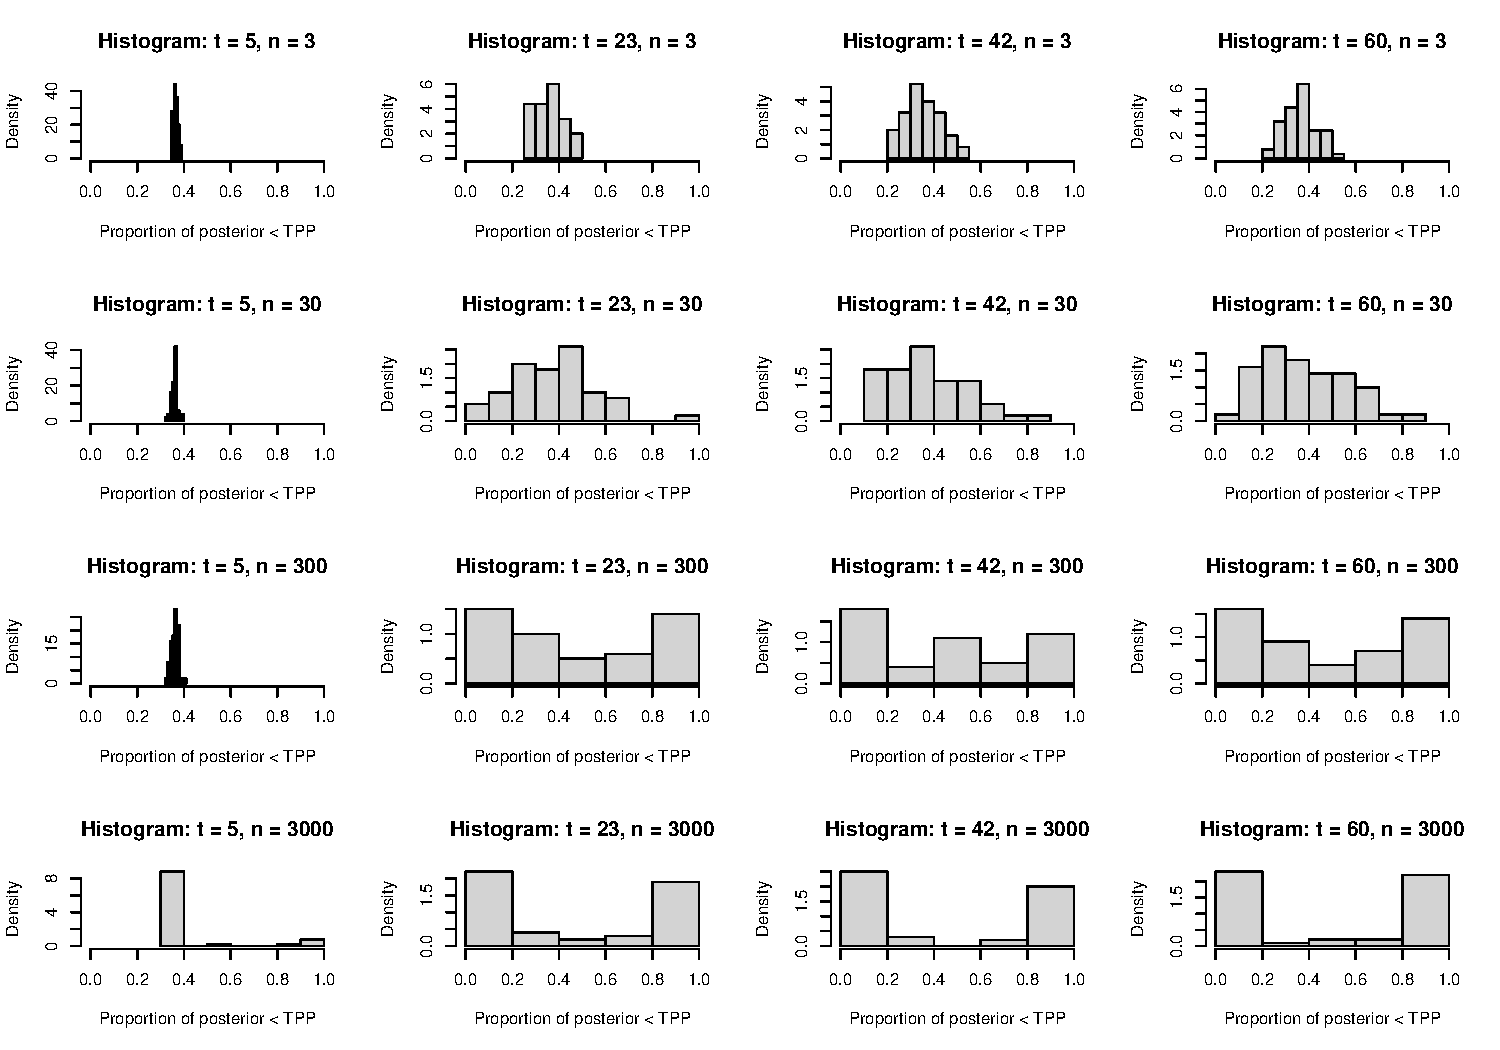
\includegraphics{DTEInterim_files/figure-beamer/unnamed-chunk-2-1.pdf}
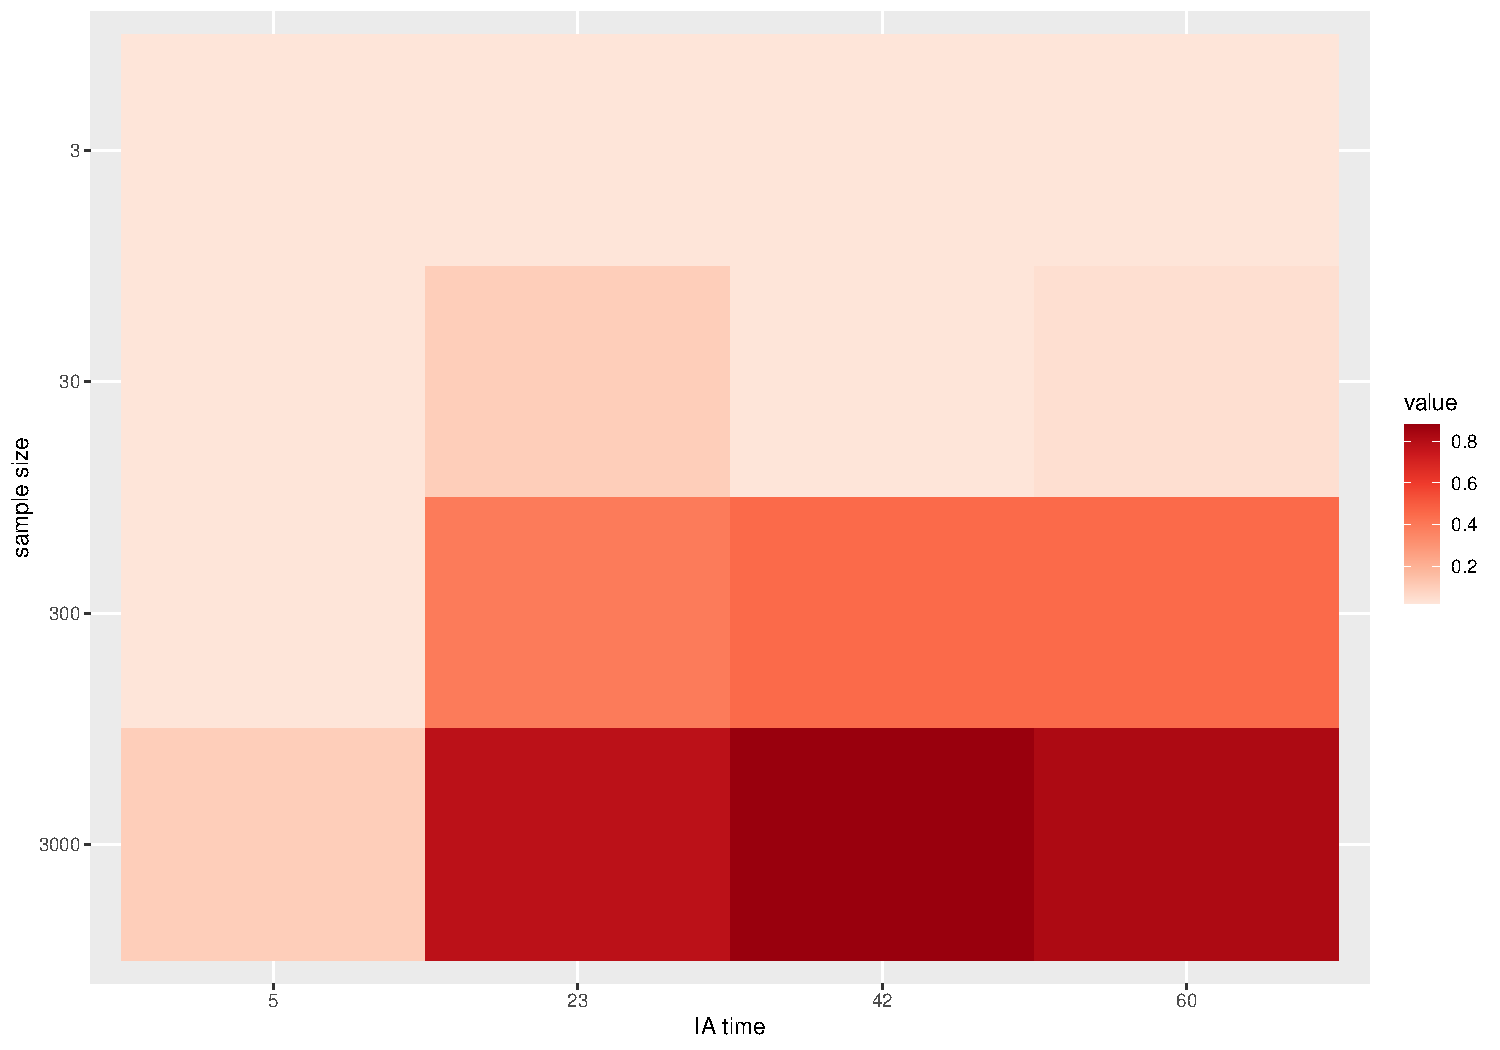
\includegraphics{DTEInterim_files/figure-beamer/unnamed-chunk-2-2.pdf}
\end{frame}

\begin{frame}{Approximation}
\protect\hypertarget{approximation}{}
We can approximate this by using the formula:

\[1.96\pm \sqrt{\frac{1}{E_1}+\frac{1}{E_2}},\]

where \(E_i\) is the expected number of events in group i.

This approximation produces the following histograms:

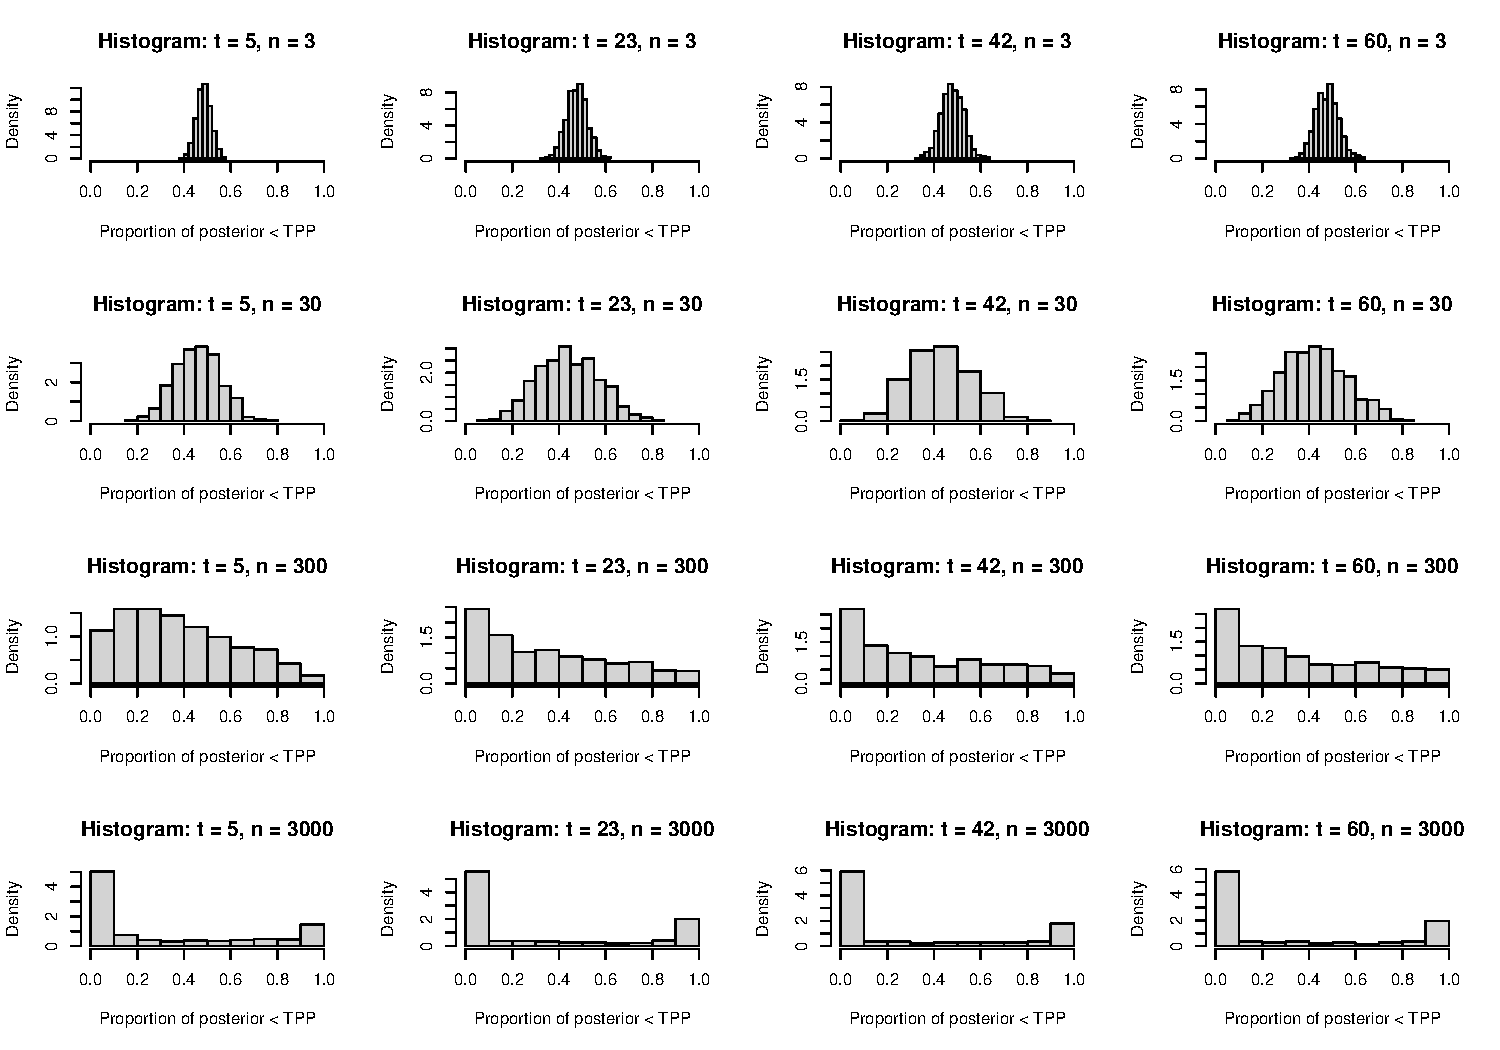
\includegraphics{DTEInterim_files/figure-beamer/unnamed-chunk-3-1.pdf}
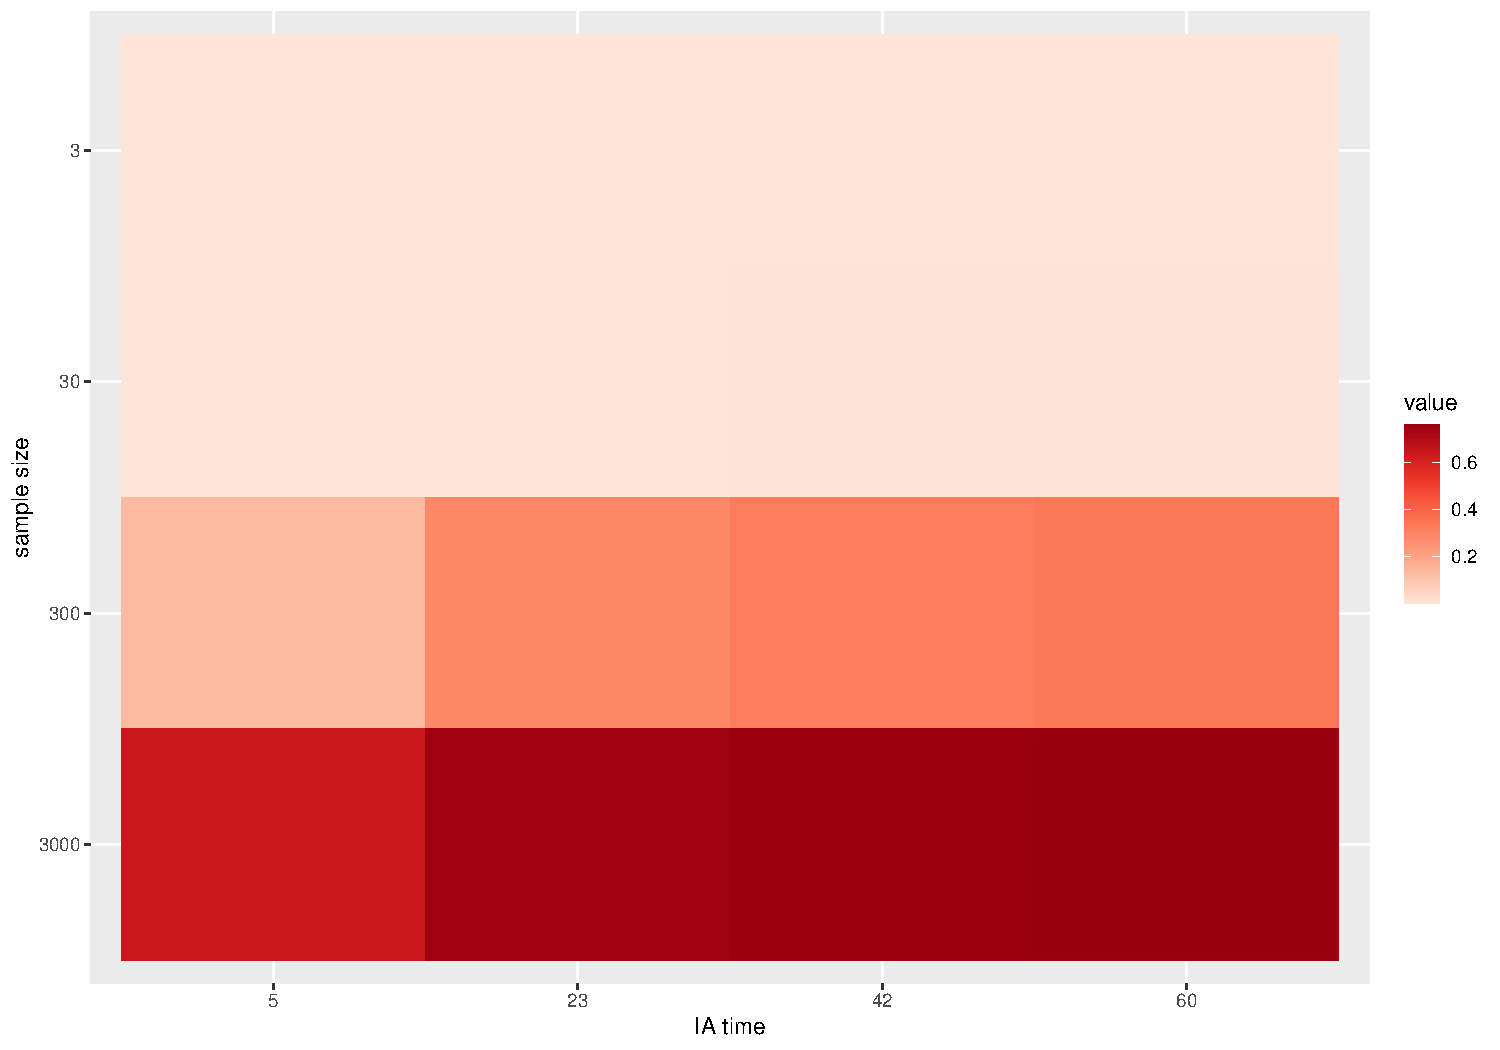
\includegraphics{DTEInterim_files/figure-beamer/unnamed-chunk-3-2.pdf}
\end{frame}

\end{document}
